% !TeX document-id = {89692b3f-10f2-4306-8854-08b16e53cfc0}
\documentclass{scrartcl}
\usepackage{enumitem}
\usepackage[utf8]{inputenc}
\usepackage[english]{proposal}
\usepackage{xcolor}
\usepackage{adjustbox}
\newcommand\todo[1]{\textcolor{red}{#1}}
\newenvironment{itemize*}%
  {\begin{itemize}%
    \setlength{\itemsep}{0pt}%
    \setlength{\parskip}{0pt}}%
  {\end{itemize}}

\addbibresource{ref.bib}
\renewcommand*{\bibfont}{\fontsize{9pt}{1.2}\selectfont}

\newcommand{\mypar}[1]{\smallskip\vspace{-0.1em}\noindent\textbf{#1.}}

\newcommand{\applicants}{\normalfont  Henrik Leopold, Hamburg \\ Han van der Aa, Mannheim \bfseries}
\newcommand{\project}{Flexible Process Discovery from User Interaction Logs Using Semantic Technology}

\renewcommand{\sectionautorefname}{Section}
\renewcommand{\subsectionautorefname}{Section}
\renewcommand{\subsubsectionautorefname}{Section}

\begin{document}

% !BIB TS-program = biber

{\raggedright{} \normalsize \bfseries 
	Project Description - Project Proposals \par 
	\applicants{} \par
	\project{} \par
	\rule{\textwidth}{0.5pt} \par
	Project Description
}

\newenvironment{nscenter}
 {\parskip=3pt\par\nopagebreak\centering}
 {\par\noindent\ignorespacesafterend}
 
 
 %++++++ SECTION 1 ++++++
\section{Starting Point}
\label{sec:startingpoint}

Process mining is widely used to discover, analyze, and improve business processes \cite{van2016data}. Traditional process mining techniques reconstruct how a process is executed by analyzing so-called event logs. These event logs are extracted from IT systems and, therefore, provide insights into how exactly processes are executed in the organization . However, this approach has an important limitation: It limits the scope of process discovery to \textit{back-end events}, i.e., secondary, indirect events that were triggered by the actual user activity \cite{diba2020extraction}. User activities that do not result in such back-end events or take place in productivity applications such as Excel, Outlook, and other desktop applications are, therefore, invisible to traditional process mining techniques. 

To avoid this problem and be able to obtain a comprehensive view on business processes, the goal of this proposal is to develop a novel technique that conducts process discovery based on \textit{user interaction (UI) logs} rather than traditional event logs. In essence, UI logs are a collection of interactions performed on GUI components such as clicks on buttons or keyboard entries in text areas \cite{Urabe21}. The advantage of UI logs is that they can be obtained for any type of business process regardless of the software applications that are used for its execution. The only requirement is that relevant activities are performed using a computer. Available \textit{logging software} is then able to extract and store relevant data such as the interaction type (e.g. click or keyboard stroke), the interaction time, and the interaction context (e.g., the affected GUI element, window title, URL, etc.) in an UI log  \cite{leno2019action}. Figure \ref{fig:example} shows a simplified excerpt of such an UI log. The events from this UI log show how a user handles order requests using the application Salesforce that are received via e-mail. 

\begin{figure}[h!]
\centering
 \begin{adjustbox}{max width=\textwidth}
\begin{tabular}{llllllll}
\hline\noalign{\smallskip}\noalign{\smallskip}
\textbf{ID} &\textbf{Timestamp}&\textbf{Event}&\textbf{Application}&\textbf{Element label}&\textbf{Element type}&\textbf{Element value}&\textbf{URL}\\
\noalign{\smallskip}\hline\noalign{\smallskip}
1&08:35.2&click&Outlook&Customer X - O123&list&Please initiate an order …&-\\\noalign{\smallskip}
2&08:35.2&click&Outlook&Customer X - O234&list&Please initiate an order …&-\\\noalign{\smallskip}
3&08:35.2&click&Outlook&Customer Y - O789&list&Please initiate an order …&-\\\noalign{\smallskip}
4&08:39.7&click&Chrome&Log in&button&-&https://www.salesforce.com/\\\noalign{\smallskip}
5&08:40.0&change&Chrome&Password&text field&-&https://login.salesforce.com/\\\noalign{\smallskip}
6&08:40.5&click&Chrome&Submit&button&-&https://login.salesforce.com/\\\noalign{\smallskip}
7&08:52.6&click&Chrome&New Account&button&-&https://com.lightning.force.com/home\\\noalign{\smallskip}
8&08:53.2&change&Chrome&New Order&text field&Customer X&https://com.lightning.force.com/acc/\\\noalign{\smallskip}
9&08:53.9&ctrl + c&Outlook &Customer X - O123&list&Please initiate an order …&-\\\noalign{\smallskip}
10&08:54.3&click&Chrome&Billing address&text field&-&https://com.lightning.force.com/acc/\\\noalign{\smallskip}
11&08:54.4&ctrl + v&Chrome&Billing address&text field&Hofstraße 14, ... &https://com.lightning.force.com/acc/\\\noalign{\smallskip}
12&08:54.9&click&Chrome&Save&button&-&https://com.lightning.force.com/acc/\\\noalign{\smallskip}
13&08:40.0&change&Chrome&Password&text field&-&https://www.facebook.com/\\\noalign{\smallskip}
14&08:42.9&click&Chrome&Log in&button&-&https://www.facebook.com/\\\noalign{\smallskip}
15&08:42.9&click&Chrome&Messenger&button&-&https://www.facebook.com/\\\noalign{\smallskip}
16&08:44.1&click&Chrome&New message&list&Hey, how are you? …&https://www.facebook.com/\\\noalign{\smallskip}
17&08:56.7&click&Outlook&Customer X - O234&list&Please initiate an order …&-\\\noalign{\smallskip}
18&08:58.2&change&Chrome&New Order&text field&Customer X&https://com.lightning.force.com/acc/\\\noalign{\smallskip}
19&08:58.6&click&Chrome&Upload files&button&CustomerX-2021-O234.docx&https://com.lightning.force.com/acc/\\\noalign{\smallskip}
\hline\noalign{\smallskip}
\end{tabular}
\end{adjustbox}
\caption{Simplified excerpt of an UI log}
\label{fig:example}
\end{figure}

A closer look a at the UI log from Figure \ref{fig:example} reveals that conducting process discovery on such a log is a complex task. Specifically, five main challenges need to be overcome: 

\begin{itemize}
\item \textit{Challenge 1: Noise filtering}: UI logs may contain events that do not relate to the actual process execution. Examples include visits to social media platforms, checking private e-mails, and ordering private items in online shops. In the UI log from Figure \ref{fig:example}, we observe a case from the first category: The user briefly switches to the social media platform Facebook to read a message before resuming the work in Salesforce. Note that not all noisy events can be recognized via the type of application or the URL. As an example consider reading a private e-mail that was sent to the professional e-mail address of the user. All these events must be properly recognized and removed since they are not part of the actual process execution. 
  
\item \textit{Challenge 2: Case identification}: One of the key requirements of process discovery algorithms is the availability of a so-called \textit{case identifier} \cite{van2016data}. This case identifier is required to relate each event from the event log to a specific execution of the process (referred to as \textit{process instance} or \textit{case}). Unfortunately, the notion of case identifier is generally missing in UI logs \cite{leno2021robotic}. To illustrate the challenge of recognizing which events in an UI log belong to the same case, again consider the events from Figure \ref{fig:example}. In the beginning of the log, we observe three events that potentially relate to three different cases. It seems that the user checks more than a single e-mail before picking up the first order. From the overall context, we can then infer that events 4 to 12 relate to the case concerned with order \textit{O123} from Customer X. This, however, can be only safely inferred from event 11 where the billing address from Customer X is entered into the system. Events 17 to 19 then relate to the case concerned with order \textit{O234} from Customer X, which we first encountered in event 2. Again, we can only indirectly infer this from the name of the file that is uploaded to Saleforce. 

\item \textit{Challenge 3: Event abstraction}: A process model that is directly derived from the events from an UI log will be very large and only contain low level events such as ``\textit{Click confirm button}'' or ``\textit{Open e-mail}". From an analytical point of view, however,  it would be desirable to include higher level events that represent actual business activities such as ``\textit{Create order}'' or ``\textit{Contact customer}''. This process of event abstraction is highly challenging since UI events constituting a business activity may not be executed consecutively and in varying ways. As an example, consider the events relating to the creation of orders \textit{O123} and \textit{O234}. The creation of the first order involves entering a billing address while the creation of the second order involves uploading a file. 

\item \textit{Challenge 4: Event labeling}: A useful process representation requires clear and expressive text labels. Therefore, once higher-level events have been identified, they still need to be labeled properly. Automatically concluding that, for instance, events 8 to 12 can be appropriately described by ``\textit{Create order}'' is considerably complex. Here it is required to recognize the overall context and the final outcome of a series of low level events.  
 
\item  \textit{Challenge 5: Model discovery}: The outcome of process discovery is typically a process model-based representation. There are, however, a plethora of different algorithms available, each having different strengths and weaknesses. So far, existing process discovery algorithms have not been applied in the context of UI logs. The challenge, therefore, is to identify which algorithm is best suited to provide the user with an effective representation of the discovered process. 
 \end{itemize}

An effective technique for discovering process models from UI logs should be able to successfully cope with all these challenges. In the following, we review the state of the art and show that these challenges are not adequately handled up to now. \todo{(We need to briefly talk about the HOW already, i.e., that we will use NLP.)}

\subsection{State of the art and preliminary work}
 
\subsubsection{State of the art} 
 \label{sec:stateoftheart}
 
The proposed project primarily relates to research on traditional process mining (using event logs) and robotic process mining (using UI Logs). Below, we briefly review these streams and highlight the gaps that exist with respect to the challenges identified above.  

\mypar{Process mining} Process mining is a family of data analysis techniques that facilitate the discovery, analysis, and improvement of business processes \cite{van2016data}. The core idea of process mining techniques is to analyze so-called \textit{event logs}. These event logs are extracted from information systems that support the execution of business processes and, therefore, capture how these processes are actually executed. Available process mining techniques serve a wide range of tasks including process discovery, conformance checking, and enhancement. Techniques for \textit{process discovery} (see e.g. \cite{gunther2007fuzzy,weijters2011flexible,leemans2013discovering}) aim to provide the user with a visual representation of the process captured in the event log. \textit{Conformance checking} techniques (see e.g. \cite{rozinat2008conformance,adriansyah2011conformance}) detect differences between the actual and intended process execution by comparing the event log with a normative process model. Techniques for \textit{enhancement} again address a variety of tasks such as predicting relevant aspects of the process execution \cite{di2018predictive} or repairing a given process model based on the event log \cite{polyvyanyy2016impact}. Many of the challenges highlighted in the two problem areas above, also play a role in these ``traditional'' facets of process mining. Specifically, process mining techniques have been concerned with the challenges of noise filtering and case identification (problem area 1) as well as the challenges of event abstraction, event labeling, and model discovery (problem area 2):
\vspace{0.2em}
\newline%
\noindent \textit{Noise filtering:} The removal of noise directly affects the quality of process models generated by process discovery techniques, as well as of other process mining results. 
Therefore, various discovery techniques take noise into account explicitly (e.g.,~\cite{weijters2003rediscovering,leemans2013discovering,van2016avoiding}), whereas there are also dedicated techniques available  for removing noise from events logs~\cite{tax2017discovering,CHENG2015138}. However, one of the key assumptions of all these techniques is that noise is highly infrequent. This is problematic in our context, since if certain process-irrelevant actions (e.g., visiting social media websites) occur on a regular basis, they would not be recognized as noisy by frequency-based techniques. 
\vspace{0.2em}
\newline%
\noindent \textit{Case identification:}  The problem of case identification in event logs is addressed by various existing techniques (cf.,~\cite{diba2020extraction} for an overview). However, they consider rather restrictive settings. The technique from Ferreira and Gillblad ~\cite{ferreira2009discovering} provide a solution for processes that do not contain loops or activity repetitions, whereas the technique from Bayomie et al.~\cite{bayomie2019probabilistic} assumes that a process model is already available. Both are assumptions that will not be met in the context of our project. 
\vspace{0.2em}
\newline%
\noindent \textit{Event abstraction:} 
The issue of event abstraction has also been discussed in the context of traditional process mining~\cite{van2020event,diba2020extraction}. Recognizing that recorded events can differ widely in their granularity, several abstraction techniques have been proposed to obtain consistent and useful event logs or process models (e.g. \cite{baier2014bridging,van2020event,de2020event}). Available techniques differ with respect to many aspects such as the type of supervision (supervised/ unsupervised), the handling of concurrency (yes/ no), and the type of output (probabilistic/ deterministic). What is currently still missing from the perspective of this project is an unsupervised technique that can can deal with the large degree of variability in UI logs and reliably recognize respective higher-level events. 
\vspace{0.2em}
\newline%
\noindent \textit{Event labeling:} 
While the problem of labeling higher-level events has been recognized and discussed in the context of process mining~\cite{van2020event,van2016enabling}, no dedicated techniques to overcome this problem currently exist. Instead, the  currently proposed solution is to delegate this task to domain experts. For our goal of automated elicitation and discovery of processes, this caveat must thus be addressed.   
\vspace{0.2em}
\newline%
\noindent \textit{Model discovery:} 
While various process discovery techniques exist (cf., \cite{augusto2018automated} for an overview), the vast majority are designed to deal with higher-level event logs. Closest to our goal is recent work on multi-level process discovery~\cite{leemans2020using}, which is the first to recognize the importance of granularity in discovery. Yet, the process models it yields lack intuitiveness, whereas it imposes strong requirements on the input logs it can handle. As such, it provides a useful foundation for our project, yet leaves a considerable gap to be addressed.

%In principle, each of the available process model discovery techniques could be used to address the model discovery challenge of this proposal. However, existing discovery techniques were designed for traditional event logs and not for UI logs. Therefore, they do not provide dedicated mechanisms to deal with the problem of granularity.  
 
% \noindent\fbox{%
%\parbox{0.985\textwidth}{%
%In summary, traditional process mining research has recognized five of the six challenges we identified for this project. Available solutions, however, are not applicable because of a limited scope, simplifying assumptions, or an insufficient degree of automation.
%}}

\mypar{Robotic process mining} Robotic process automation (RPA) is a technology that aims to automate repetitive human work. The core idea is to let software robots (or bots) mimic the actions of a human directly in a GUI \cite{SYED2020103162}. A key requirement of RPA is to actually identify automatable tasks.  Recognizing this, the research domain of robotic process mining (RPM) has emerged in recent years \cite{leno2021robotic}. The goal of RPM techniques is to automatically identify automatable routines based on UI logs. 
By doing so, RPM faces several challenges with the ones identified for the proposed project, primarily with respect to of noise filtering and case identification from Problem area 1:   
\vspace{0.2em}
\newline%
\noindent \textit{Noise filtering:} 
Also in the context of RPA, noisy events such, such as social media visits, need to be removed from UI logs, since they should not become part of automated procedures. However, effective solutions for noise removal from UI logs are missing. While noise removal techniques from traditional process mining (see above) are generally applicable, their limitations for removing noise from UI logs have also been recognized \cite{leno2021robotic}. 
As a solution, some authors propose supervised noise removal based on an existing process model \cite{agostinelli202111} or they suggest using rules \cite{bosco2019discovering,leno2020identifying}. However, such process models cannot be expected to be available in the context of our project, whereas rule-based approaches are too rigid to deal with the flexibility of real-world UI logs.
\vspace{0.2em}
\newline%
\noindent \textit{Case identification:} The identification of cases in RPM conceptually differs from case identification in traditional process mining. The underlying assumption in RPM is that cases do not overlap and, thus, that case identification can be achieved by splitting the log into segments. 
Researchers have proposed manual, supervised, and unsupervised approaches for this segmentation task. Urabe et al.~\cite{urabe2019visualizing} introduced a manual approach that visualizes the UI log using a graph and, in this way, supports the user in identifying segment boundaries. Agostinelli et al. \cite{agostinelli202111} proposed a supervised approach, requiring a process model, that leverages trace alignments from conformance checking. 
%This approach, however, requires a Petri net representing the underlying process as input. 
An unsupervised approach was introduced by Leno et al. \cite{leno2020identifying}. They construct a control-flow graph from the UI log and use back edges detection to identify segment boundaries. Another, very recent, unsupervised approach from Urabe et al. \cite{Urabe21} leverages the concept of co-occurrence from topic segmentation in natural language processing to segment the UI log. Despite the potential of these techniques, 
the assumption that cases are executed in a strictly sequential manner does not hold for many real-world settings, in which users may work concurrently on different cases (cf., \autoref{fig:example}).



\subsubsection{Preliminary work}
\label{sec:preliminarywork}

The applicants, Prof.\ Leopold and Prof.\ Van der Aa, have published various works that relate to the proposed project. Both applicants have considerable expertise when its comes to the use of natural language processing (NLP) for the purposes of process analysis, through individual as well as joint works, which forms a key component in the proposed solutions.
Furthermore, the project relates to individual experience of the applicants with respect to the analysis of low-level event data (Prof.\ Van der Aa) and to the understandability of process representations (Prof.\ Leopold):


\mypar{NLP for process analysis}
The applicants have developed approaches for the extraction of semantic information, such as actions and business objects, from activity labels in process models~\cite{leopold2013detection,leopold2019using} and data attributes in event logs~\cite{rebmann2021extracting}.
This expertise shall provide the foundation for event annotation in UI logs, a primary task in the proposed project. A key distinction, though, is that the existing works are designed to deal with short fragments (such as ``\emph{create purchase order}''), whereas the project at hand shall also deal with larger texts, such as e-mails. In that regards the applicants can also build on their expertise when extracting process information from textual process descriptions, e.g., for the recognition of process constraints~\cite{van2019extracting,winter2020assessing} and for querying~\cite{leopold2019searching}. Here, a key distinction is that those approaches were designed for process-oriented texts, whereas the proposed project shall also deal with texts that are not structured in this manner.

Recently, the applicants showed the potential of employing semantic information in process mining when using extracted business objects and actions for the purposes of \emph{semantic anomaly detection}~\cite{van2021natural}. Specifically, the work demonstrates that NLP can be leveraged to detect process behavior that violates commonsense rules. This provides a novel angle for anomaly detection in comparison to existing works, which deem process behavior to be anomalous when it is infrequent.
This work shall provide a starting point for the noise filtering that is required in the proposed project. However, next to the recognition of behavioral anomalies, the project also requires techniques that are specifically designed to recognize and remove non-business related events.




\mypar{Analysis of low-level event data} 
Prof.\ Van der Aa has worked on several projects involving the analysis of low-level event data in both event logs and streams, which have clear similarities to the data granularity used in the proposed project.
Existing work relates to the identification of key event patterns in streams~\cite{vanderaa2021cep}, which can provide a basis for the recognition of behavioral regularities for case identification.
Furthermore, experience on the efficient handling of large amounts of low-level events~\cite{zhao2021eires} can aid the computational efficiency of approaches developed for the proposed project, especially for tasks such as case identification and log abstraction that require global optimization.
Finally, ongoing work on log abstraction with guarantees~\cite{rebmann2021icdesubm} can be used as a starting point for the meaningful abstraction of UI logs, since the characteristics of these logs can be used to guide the abstraction task, e.g., by ensuring that events from different systems are not grouped together.

\mypar{Understandability of processes}
Prof.\ Leopold has worked extensively on the topic of process model understandability, especially from a linguistic angle. Among others, he has developed techniques for automatically recognizing and correcting linguistic problems in process models that negatively affect the understandably of process models~\cite{leopold2013detection,leopold2012refactoring,pittke2015automatic}. In this context, he has also proposed a technique that attempts to automatically determine names for (to be aggregated) process model fragments \cite{leopold2014simplifying}.  The challenge of labeling events that result from event abstraction in event logs is conceptually highly similar to labeling activities that result from activity abstraction in process models. However, the technique from \cite{leopold2014simplifying} relies on the specifics of event-driven process chains (EPCs) and, therefore, cannot be transferred to labeling higher-level events. Nonetheless, these works provide important input for the challenges of problem area 2. The technical aspects represent an important basis for the challenges of event abstraction and activity labeling. The experience collected with user experiments, for instance in \cite{pittke2015automatic}, will help us to successfully complete the challenge of process discovery and representation. 


\subsection{Project-related publications}
 \todo{Maximum 10 publications. Probably good to also include some we wrote separately. Let's briefly discuss this.}

\noindent \textbf{Articles published by outlets with scientific quality assurance, book publications, and works accepted for publication but not yet published}\\[6pt]
\textit{Journal articles:}
\begin{enumerate}[leftmargin=*]
\item \fullcite{van2021natural}
\item \fullcite{van2019efficient}.
\item \fullcite{leopold2019using}.
\item \fullcite{vanderaa2018checking}.
\item \fullcite{meilicke2017overcoming}.
\end{enumerate}
\textit{Conference papers:}
\begin{enumerate}[resume,leftmargin=*]
\item \fullcite{rebmann2021extracting}
\item \fullcite{van2019extracting}.
\item \fullcite{van2018challenges}.
\item \fullcite{van2016dealing}.
\item \fullcite{leopold2015towards}.
\end{enumerate}

 % ++++++ SECTION 2 ++++++
\section{Objectives and work programme}
 \subsection{Anticipated total duration of the project}

The anticipated duration of the project is three years (36 months).

\subsection{Objectives}
\label{sec:objectives}

The goals of the project are 

\begin{itemize}
\item to develop a technique that can automatically ...   

\item to show the practical value ... 
\end{itemize}

We will approach the \textit{first goal} by defining a novel technique that combines NLP with .... Figure \ref{fig:approach} gives an high-level overview of the proposed architecture. It shows that the proposed technique consists of four main steps.    \todo{(The big question here is: Is it lame to have a 1:1 link between challenges and steps / work packages? I feel we would benefit from a setting where the challenges are part of something bigger.)}

\begin{figure}[h!]
\centering
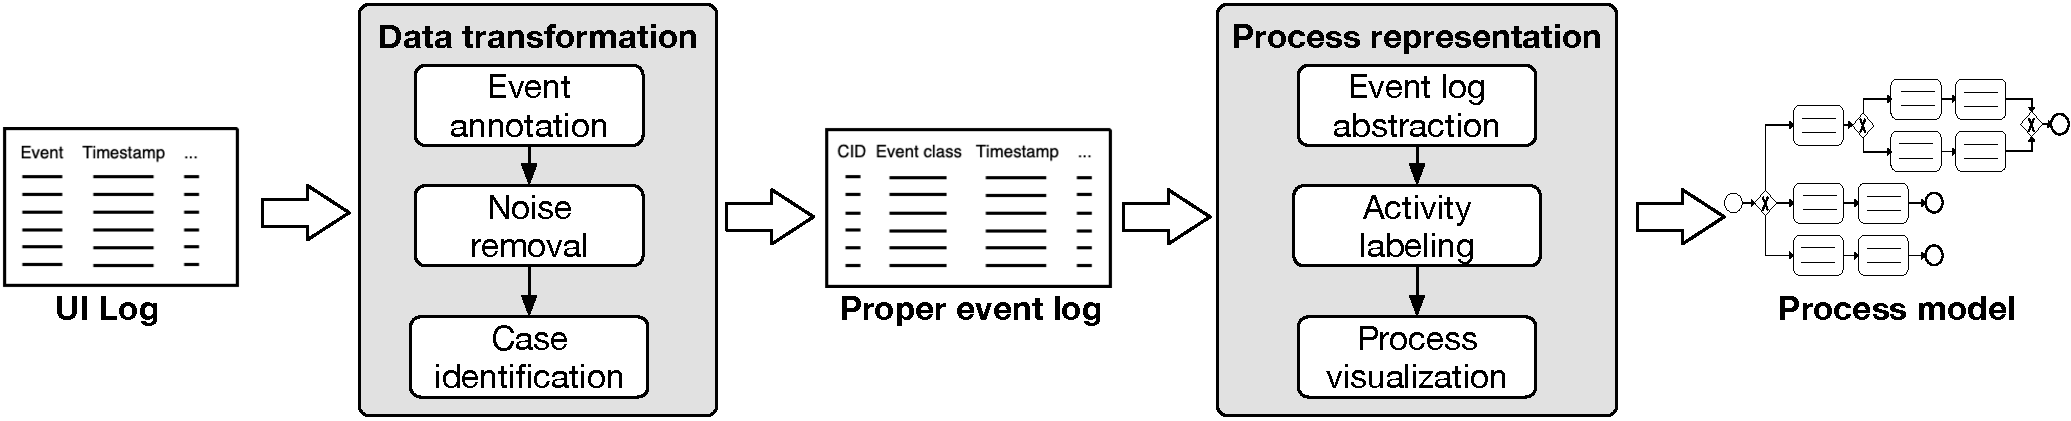
\includegraphics[width=\textwidth]{figures/overview.pdf}
\caption{Overview of the proposed project}
\label{fig:approach}
\end{figure}




%The input for the technique is a set of social media posts and a set of event logs\footnote{Note that the technique does not require more than a single event log, but is simply able to handle several event logs.}. 
%The \textit{first step} of the technique is concerned with identifying and extracting weaknesses in the social media posts. This will be achieved by building on NLP tools such as dependency parsers and sentence classification techniques (see work package 1, Section \ref{sec:wp1}). The goal of the \textit{second step} is to identify the links between the identified weaknesses and the events from the event logs. To achieve this, we will  
% characterize the links between all possible weakness-event pairs by using different perspectives of similarity (see work package 2, Section \ref{sec:wp2}). Based on these link characterizations, we will then use optimization rules specified in a Markov Logic formalization to compute the most likely correspondences between weaknesses and events. The rules of the Markov Logic formalization may, for instance, specify that a weakness can only be linked to an event if the timestamp of the associated social media post indicates that the event occurred before the post was created. The definition of appropriate rules will be one of the key tasks of this project (see work package 3, Section \ref{sec:wp3}). The \textit{third step} is concerned with clustering and ranking the weaknesses. The purpose of clustering weaknesses is to recognize whether several weaknesses that are linked to a single event relate to the same \textit{weakness class}. For example, several customers may complain about waiting too long before receiving a voucher. Therefore, we would consider \textit{voucher waiting time} as a weakness class. The purpose of then ranking these weakness classes is to provide an indication of where to start with the improvement initiative. The idea is that highly ranked weakness classes are more frequent and more severe than lower ranked weakness classes. After clustering and ranking, we, therefore, can generate a weakness report that can serve as input for a process improvement initiative (see work package 4, Section \ref{sec:wp4}). 
 
%We will approach the \textit{second goal} of the project by implementing the automated technique defined in work packages 1 through 4. Moreover, we will systematically evaluate the implemented technique by applying it to different real-world data sets. While social media posts are publicly available and can be efficiently obtained via APIs\footnote{See e.g. https://developer.twitter.com/en/docs.}, event log data is harder to obtain. However, there are a number of relevant event logs that are publicly available and that we plan to use as a starting point:
%\begin{itemize}
%\item \textbf{BPI Challenge 2016}: This event log  originates from the International Business Process Intelligence Challenge from the year 2016. It contains events from the Dutch Employee Insurance Agency (UVW), which handles employee insurances and provides labor market-related services in the Netherlands. This log is well-suited for the purposes of this project because it is customer-oriented and contains text data (similar to social media posts) about customer complaints in English.
%\item \textbf{BPI Challenge 2019}: This event log originates from the International Business Process Intelligence Challenge from the year 2019. It contains (English) events from the purchase order handling process of AkzoNobel, a large multinational company with over 50 subsidiaries in the area of coatings and paints. While this log well-suited for the purposes of this project because it is customer-oriented, it does not come with textual resources created by customers. However, we will obtain relevant data from Twitter and, in this way, manually complement the log. 
%\end{itemize} 

%The implementation of the proposed technique will be conducted in Python and based on the PM4Py process mining framework\footnote{https://pm4py.fit.fraunhofer.de/} (work package 5, Section \ref{sec:wp5}). By manually creating gold standards for our evaluation data sets, we will test our technique with respect to its extraction, alignment, and clustering capabilities. We will use the evaluation results both during the project for improving our technique and at the end of the project in the context of a summative evaluation (work package 6, Section \ref{sec:wp6}). In the following, we describe the work packages in detail. Note that we provide the estimated duration of each work package in project months (PM) in the title of each work package. 

\subsection{Work programme including proposed research methods}

\todo{Open questions / points:}
\begin{itemize}
\item \todo{I feel we need to find a real UI log or we should probably mention that we will create one. Given available software, this is not a big deal, but currently this topic is not covered.}
\item \todo{We need to streamline the terms: technique, approach, mechanism, component. \textbf{Discussed but need to implement}}
\end{itemize}

\mypar{Package structure} We divided the work programme into two work streams (WS1 and WS2) and a total of six work packages (WP1 to WP6). WS1 will be led by the University of Mannheim and consists of WP1 to WP3. WS2 will be led by the Kühne Logistics University and consists of WP4 to WP6. We have designed the two work streams in such a way that they can be executed independently from each other. We achieved this by making sure that WP4 can build on publicly available, traditional event logs until the first results from WP3 are available. Therefore, both work streams can start in parallel. 

\mypar{Research method} We will achieve our objectives through the design, implementation, and evaluation of novel process mining approaches. The implementation of the proposed approaches will be conducted in Python, based on the \textit{PM4Py} process mining framework\footnote{\url{https://pm4py.fit.fraunhofer.de/}}. The evaluation will be primarily based on publicly available real-world event logs\footnote{\url{https://www.tf-pm.org/resources/logs}}, whereas WP6 will focus on empirical usefulness trough user experiments. By manually creating gold standards for our evaluation data sets, we will test the techniques developed in each WP with respect the specific WP objective. We will use the evaluation results both during the project for improving our techniques and at the end of the project in the context of a summative evaluation at the end of WP6. 
 
\subsubsection{Work package 1: UI log enrichment (X PM)}
\label{sec:wp1}

We have already shown that UI logs contain a number of relevant attributes for each event. While these attributes may substantially differ per event in a real-world UI log, there is one attribute that is always missing in UI logs in comparison to traditional event logs: an event label revealing what precisely happened. To illustrate this, consider the shortened version of our UI log in \autoref{fig:example_short}. In a traditional event log, event 1 would probably carry a label such as ``\textit{Receive order}''. In the present UI log, we see that the event was a ``\textit{click}'' on a ``\textit{list}'' in the application ``\textit{Outlook}''. That this click relates to receiving an order from a customer can only be inferred from the associated e-mail. Events 4 and 14 also highlight the importance of proper event labels for classifying events. Looking at the key attributes \textit{Event}, \textit{Application}, \textit{Element label}, and \textit{Element type}, they seem to be identical. However, in fact, event 4 leads the user to a log in screen (the password entry succeeds the event), while event 14 completes the log in process (the password entry precedes the event). Proper labels could have clarified this difference. Here, only the \textit{URL} attribute helps to recognize that the specific application context differs. Unfortunately, the application in which an event occurred is sometimes hard to determine. For example, consider events 4, 7, and 13. According to the UI log, these events all occurred in the context of the application ``\textit{Chrome}'', i.e., an Internet browser. However, a brief analysis of the respective URL attributes reveals that event 4 relates to Salesforce and event 13 relates to Facebook. The fact that also event 7 relates to Salesforce is actually hard to identify since the URL structure of Salesforce changes once the user has logged into the application. Given that we intend to build on the semantics of the UI log events, we need to respectively enrich the raw event data from the UI log such that it is clear \textit{what} happened and \textit{where}. 

\begin{figure}[h!]
\centering
 \begin{adjustbox}{max width=\textwidth}
\begin{tabular}{llllllll}
\hline\noalign{\smallskip}\noalign{\smallskip}
\textbf{ID} &\textbf{Timestamp}&\textbf{Event}&\textbf{Application}&\textbf{Element label}&\textbf{Element type}&\textbf{Element value}&\textbf{URL}\\
\noalign{\smallskip}\hline\noalign{\smallskip}
1&08:35.2&click&Outlook&Customer X - O123&list&Please initiate an order …&-\\\noalign{\smallskip}
...&...&...&...&...&...&...&...\\
4&08:39.7&click&Chrome&Log in&button&-&https://www.salesforce.com/\\\noalign{\smallskip}
5&08:40.0&change&Chrome&Password&text field&-&https://login.salesforce.com/\\\noalign{\smallskip}
6&08:40.5&click&Chrome&Submit&button&-&https://login.salesforce.com/\\\noalign{\smallskip}
7&08:52.6&click&Chrome&New Account&button&-&https://com.lightning.force.com/home\\\noalign{\smallskip}
...&...&...&...&...&...&...&...\\
13&08:40.0&change&Chrome&Password&text field&-&https://www.facebook.com/\\\noalign{\smallskip}
14&08:42.9&click&Chrome&Log in&button&-&https://www.facebook.com/\\\noalign{\smallskip}
15&08:42.9&click&Chrome&Messenger&button&-&https://www.facebook.com/\\\noalign{\smallskip}
...&...&...&...&...&...&...&...\\
\hline\noalign{\smallskip}
\end{tabular}
\end{adjustbox}
\caption{Shortend version of UI log from \autoref{fig:example}}
\label{fig:example_short}
\end{figure}

\mypar{Semantic annotation - What} Available process analytics techniques leveraging semantics (e.g., \cite{leopold2012probabilistic,leopold2015_jss,van2021natural}) typically expect that each event can be associated with at least one \textit{action} and at least one \textit{business object}. Building on the example introduced above, the action for event 1 is ``\textit{receive}'' and the business object is ``\textit{order}''. While there are several techniques to derive actions and business objects from labels \cite{leopold2012refactoring,leopold2019using,rebmann2021extracting}, we need to infer these components from the available UI attributes. Therefore, we will develop a process-specific feature extraction technique, which identifies those textual attributes that have the specific roles of actions and business objects. To achieve this, we will combine and adapt existing techniques for the recognition of semantic process components in textual attributes~\cite{rebmann2021extracting} and the extraction of actions from free-text log attributes~\cite{gupta2020analyzing}. Specifically, we will first use graph-based topic discovery algorithms, such as CorePhrase \cite{hammouda2005corephrase}, to detect which attributes carry relevant information. Then, we will use a tagging mechanism based on BERT \cite{Devlin2019} to identify relevant actions and business objects. 

\mypar{Semantic annotation - Where} In traditional event logs, the application in which an event occurred is typically clear. That is, because the application itself records the occurrence of the event. In UI logs, the recording of the event is conducted independently of the used application(s). While the active application is captured in the \textit{application attribute} of the UI log, more and more business applications are browser-based (e.g. Salesforce, Office 365, Basecamp). Hence, the specific \textit{sub application} of many events must be inferred from the associated URL. To achieve this, we mainly build on string matching techniques. First, we check whether the application from the \textit{application attribute} is an Internet browser. This is accomplished by consulting Wikipedia via the MediaWiki Action API\footnote{\url{https://www.mediawiki.org/wiki/API:Main_page}}. Second, in case the application is an Internet browser, we resolve the URL via string matching. To illustrate this, consider event 4 from \autoref{fig:example}. After removing URL-specific prefixes and suffixes, we obtain ``\textit{salesforce}'', which can be easily verified as a business application using Wikipedia. For events where this strategy does not deliver a conclusive result, we look at the event context. For example, for event 7, the string matching strategy is unlikely to deduce that this event occurred in Salesforce. However, when looking at log context, we can clearly identify a number of sub applications, such as Salesforce (from event 4) and Facebook (from event 13). Although the URL of event 7 is rather cryptic, a string matching against these two available options, would clearly identify Salesforce as the most likely sub application. In this way, we resolve URLs and enrich the UI log with the specific sub application in which each event occurred.  

\mypar{Outcome} The outcome of this work package is a technique the enriches the original UI log with three new attributes: \textit{action}, \textit{business object}, and \textit{sub application}. These additional attributes serve as an important basis for the semantic analyses in the subsequent work packages.  


\subsubsection{Work package 2:  Noise removal (X PM)}
\label{sec:wp2}

UI logs often contain events that do not relate to the business process under investigation, such as events related to private activities (e.g., checking Facebook) or to non-related business activities (e.g., filing a reimbursement form of a business trip).
Given that process mining techniques assume that the events in a log relate to a single process, these irrelevant events, also referred to as \emph{noise}, need to be identified and removed from a UI log.

While various noise detection techniques already exist (cf., \autoref{sec:stateoftheart}), these  inherently approach noise detection from a different angle. Particularly, they aim to detect process behavior that stands out in terms of frequency (such as rare occurrence of an order being accepted before it is created), i.e., they try to \emph{detect events that are behavioral anomalies}, e.g., caused by recording errors.
Instead, when dealing with UI logs, we need to \emph{detect events that do not relate to the process at hand}. 

\mypar{Semantic noise detection}
Therefore, to approach this task, we propose to develop a semantic noise detection approach tailored to the specifics of UI logs, which aims to classify events as \emph{process relevant} or not. 
To achieve this, we transform the textual attribute values associated with each event into a feature vector, after applying standard preprocessing steps such as lemmatization and stop-word removal. In this manner, we encode both general event information in features, as well as process-specific information extracted in the previous step, i.e., the event's action, business object, and system.

Once events are transformed in such feature vectors, noise identification can be approached as either a single-class or a two-class classification problem, using state-of-the-art text classifiers, such as a fine-tuned BERT~\cite{Devlin2019} model. The former involves training a classifier that recognizes which events are related to a specific process, e.g., by assuming that the majority of events in a UI log are related to that. While such an approach thus would not require any user input, the classification accuracy may be improved in a two-class setting, where users explicitly label some events as process relevant and irrelevant, so that few-shot learning techniques can be employed~\cite{yu2018diverse}.

Although such classifiers can be employed with just a UI log as input, we will also incorporate mechanisms that allow user to provide additional domain-specific information about the process at hand, such as textual documentation or (high-level) process models, which can help the classifier to better distinguish process relevant from irrelevant events.

\mypar{Outcome}
The outcome of this work package is a classification approach that identifies irrelevant events in a UI log. The approach will be applicable without requiring any additional user input, though users may improve the approach's accuracy through manual labeling of events, as well as by supplying further process-specific artifacts (e.g., a process model) as input.
%This work package focuses on the classification of events in a UI log and the subsequent identification and  removal of irrelevant, i.e., noisy, ones.
%
%\mypar{Event classification}
%\todo{maybe this should be a separate work package? since it also comes with some particular challenges}
%Process mining techniques assume that each event in a log is associated with a particular event class, denoting the action to which the event corresponds~\cite{van2016data}, such as ``\emph{accept order}'' or ``\emph{pay invoice amount}''.
%However, such event classes are not readily available for UI logs. Rather, as shown in  \autoref{fig:example}, events are characterized by various attributes in their payload, which jointly indicate the type of step that is being performed. 
%%For instance, in the form of  the respective application (e.g., Outlook or Chrome) and other details, such as the specific element in the application (e.g., an e-mail or a particular window) and relevant values (e.g., the subject and content of an e-mail). 
%To transform a UI log into an event log that can be employed in process mining, 
%each event needs to be assigned a specific event class based on its payload attributes, which may differ across UI logs or even for different events in the same log. For example, we strive to recognize that certain e-mails refer to the \emph{creation of an order}, whereas other e-mails may correspond to the \emph{handling of an order}. Though these are  two distinct process steps, they nonetheless involve the same application (e.g., Outlook), element (a particular e-mail), and likely the same e-mail subject. Therefore, we need to recognize that the content of the e-mail, as well as its position in a log, relative to related events, determine the event class in this case.
%
%To perform this classification, we recognize that process steps  can be primarily characterized by a combination of a business object (e.g., an \emph{order} or a \emph{ticket}) and an action applied to the object (e.g., \emph{create} or \emph{handle})~\cite{ref}. 
%To recognize these two components in UI events, we aim to combine and adapt existing techniques for the recognition of semantic process components in textual attributes~\cite{rebmann} and the extraction of actions from free-text log attributes~\cite{gupta2020analyzing}. Afterwards the identified event classes can be refined or grouped by employing techniques for the recognition of duplicate~\cite{ref} or polluted event labels~\cite{ref}.
%
% 
% 
% \mypar{Noise removal}
%
%\begin{itemize}
%\item Would be great to go beyond rules here. 
%\item Type 1: Repetitive actions, actions without any effect, and actions that overwrite past actions. 
%\item Type 2: Non-business related stuff: Facebook etc. However, also irrelevant e-mails.
%\item Can we use some sort of semantic angle here? Not sure whether we can determine the domain of a process and just kill anything that is unrelated or so. 
%\end{itemize}
%
%\mypar{Outcome}

\subsubsection{Work package 3: Case identification (X PM)}
\label{sec:wp3}

Once the irrelevant events have been filtered out of a UI log, we next need to recognize which events belong to the same process instance, e.g., to the same customer order or service ticket, a task referred to as \emph{case identification}.

Existing techniques that address this task in general process mining settings primarily base the identification on co-occurrence statistics, which reveal behavioral regulations in an event log (cf., \autoref{sec:stateoftheart}). While such techniques work well for relatively structured settings, their performance deteriorates for event logs stemming from more flexible environments in which the execution of several cases overlaps, such as e.g., seen in the example of \autoref{fig:example}, the first three events each start a new process instance, by initiating three different orders in a batch-like manner.

\mypar{Instance-based event matching}
Recognizing this challenge, this work package sets out to develop a new approach for case identification, tailored to the specifics of UI logs, by building on semantic matching technology.
Specifically, to determine the likelihood that events belong to the same case from a semantic viewpoint, e.g., because both refer to a same order ID or mention the same customer name, we frame the comparison of the events as an \emph{instance-based schema matching} task. For this, we recognize that events stemming from a particular application can be represented as instance in a particular schema (characterized by their payload attributes), enabling the application of existing matching techniques (cf., \cite{somerefs}).

\mypar{Optimization} Having obtained similarity scores between individual events, these scores can then be used together with behavioral regularities identified by existing techniques~\cite{ref}, and cardinality constraints (e.g., each event belongs to exactly or at most one case), to establish an optimization problem, specifically using Markov logic formulation. By solving this problem, we will obtain an event grouping that maximizes the semantic similarity and respects the identified behavioral regularities.

\mypar{Outcome}
The outcome of this work package is a case identification approach that assign case identifiers to the events in a (filtered) UI log, such that the new log encompasses a number of cases, each corresponding to a sequence of events related to the same process instance.


\subsubsection{Work package 4: Log abstraction (X PM)}
\label{sec:wp4}

UI logs comprise low-level event data, in which each event corresponds to a small action performed by a user. This fine-granular nature makes the data unsuitable for meaningful process analysis. This particularly holds for process discovery, since the application of discovery techniques on low-level event logs yields so-called \emph{spaghetti models}, as e.g., depicted in \textbf{figure}.

To tackle this issue, log abstraction is a pre-processing technique to lift the event sequences of a log to a more abstract representation, by grouping low-level events into high-level activities. Existing techniques for log abstraction (cf., \textbf{[6], [7]}) differ in the adopted algorithms and employ, for instance, clustering of events based on temporal information \textbf{[8]} or the detection of predefined patterns [9]. Yet, their focus is on how the abstraction is conducted, rather than what properties the abstracted log shall satisfy. Without dedicated control on the result of log abstraction, however, it is hard to ensure that an abstraction is appropriate for a particular context or specific analysis goal.
This is particularly problematic in the context of UI logs, since these have clear characteristics that should guide the log-abstraction task.

\mypar{Constraint-driven log abstraction}
To overcome this limitation, we propose to develop an approach for \emph{constraint-driven log abstraction}, which it supports a declarative characterization of the properties the abstracted log shall adhere to, in order to be meaningful for downstream analysis. While our approach shall support a broad range of constraint types, common ones to impose in the context of UI logs are for instance constraints that ensure that each high-level activity only comprises events that stem from the same application (to ensure semantic cohesion) or occurred within a certain timespan of each other (to ensure behavioral cohesion). 

Given such a set of user-defined constraints, our approach aims to identify an optimal log abstraction, which groups together low-level event classes into high-level activities, such that a certain distance function, quantifying the behavioral and semantic similarity of events in an activity, is maximized, while still meeting the imposed constraints.

\mypar{Solution algorithms}
to guarantee an optimal solution, we will initially develop an algorithm for exhaustive log abstraction. Yet, striving for more efficient processing, we will also provide a heuristic algorithm that is guided by behavioral dependencies found in the log, e.g., by recognizing certain event classes that shall never be grouped into a single activity, due to their relative positions in traces.
As such, this heuristic algorithm shall aim to considerably improve the algorithm's computation time, with limited impact on the quality of the obtained results.

\mypar{Work package outcome}
\todo{discuss if this is about the outcome of the approach or the outcome of the package, which is the approach itself}


\subsubsection{Work package 5: Event labeling (X PM)}
\label{sec:wp5}

The value of a discovered process model highly depends on the quality of the event labels in the underlying event log. That is, because the event labels are included in the discovered model and, hence, form the basis for what a human can understand about the process \cite{mendling2010activity,Leopold2013Book}. In the context of process modeling, the importance of clear and informative labels has led to a large body of literature concerned with labeling guidelines \cite{mendling2010seven,leopold2015learning} and their automatic enforcement \cite{leopold2013detection,becker2009towards}. The bottom line is that process model activity labels should contain an action provided as an imperative verb (e.g. ``\textit{create}" or ``\textit{send}'') and at least one business object provided as a noun (e.g. ``\textit{order}'' or ``\textit{e-mail}''). Additional information can be provided at the end of the label if required. Examples of proper labels following these rules are ``\textit{Create order}'' or ``\textit{Send e-mail to customer}''. The challenge in the context of this work package is to automatically generate such meaningful labels from for each group of UI events that has been created in the previous work package. To illustrate this, consider the events 4, 5, and 6 from the UI log in Figure \ref{fig:example}. A possible proper label capturing the semantics of these three UI events could be ``\textit{Log into Salesforce}". Automatically generating such a \textit{higher-level label}, however, is highly complex since it requires to infer an overarching activity from the action, business object, and (sub) application attributes.

\mypar{Linguistic relation detection} To generate higher-level labels, we combine the behavioral and the semantic perspective of the process execution. The general observation is that there are different strategies to infer higher-level labels depending on the nature of the considered events. Building on the observations from early work on process model name generation \cite{leopold2014simplifying}, we distinguish three specific strategies: 1) outcome-oriented labeling, 2) decision-based labeling, and 3) holonym-based labeling. The \textit{outcome-oriented labeling} strategy can be applied if the considered set of UI events has a clear result that can be used to described the previous steps. As an example, again consider events 4, 5, and 6 from \autoref{fig:example}. While these three events relate to different specific activities, they can be perfectly summarized by referring to event 4 only, i.e., ``\textit{Log into Salesforce}". The \textit{decision-based labeling} strategy builds on the fact that many processes require the user to make decisions such as rejecting or accepting an offer from a customer. If a considered group of events contains an action that can be related to a decision, this decision will be also used to label the event, even if making the decision is associated with a number of additional events. A possible label for the above-introduced example could be ``\textit{Decide about customer offer}''. The \textit{holonym-based labeling} strategy considers a situation where all (or most) events of the considered event group jointly contribute to a higher-level event. In linguistics, a \textit{holonym} is a term that has a part-of relation with a number of \textit{meronyms}. For example, a ``\textit{finger}'' is a meronym of the holonym ``\textit{hand}''. In the context of the holonym-based labeling strategy, we extend the notion of holonymy to events. This means that the attribute values of action, business object, and (sub) application of events are considered meronyms and we aim to detect the holonym describing the higher-level event. As an example, consider events 11, 12, and 13 from \autoref{fig:example}. While these events are essentially copy and paste operations, they all contribute to a higher-level event that could be described as ``\textit{Create customer account in Salesforce}''. Existing work in the area of process analytics has tried to address the problem of holonymy detection by building on the taxonomy WordNet \cite{leopold2014simplifying}. While WordNet is useful to detect general-purpose holonymy relations (such as the one between ``\textit{finger}'' and ``\textit{hand}''), it does not help to detect more complex and domain-specific relations. Therefore, we will leverage techniques from ontology learning \cite{al2020automatic,wong2012ontology} to automatically derive holonymy relations from general and domain-specific text corpora.    

\mypar{Outcome} The outcome of this work package is a technique that creates an event log with properly labeled higher-level events, i.e., labels consisting at least of an action and a business object. This event log serves as input for the technique from work package 6. 

\subsubsection{Work package 6: Visualization (X PM)}
\label{sec:wp6}

The final step is concerned with the visualization of the process captured in the UI log. In traditional process discovery, this is achieved by generating respective process models. Depending on the employed discovery algorithm, the resulting process model is a simple directly-follows graph \cite{van2019practitioner}, a Petri net \cite{van2004workflow}, a BPMN model \cite{conforti2016bpmn}, or a process tree \cite{leemans2013discovering}. While each algorithm and output representation come with advantages and disadvantages, there is no specific discovery technique available for the UI log generated in WP1 to WP5. The specific challenge is that the original level of granularity of the UI log is not appropriate for visualization since the number of events is too high. Yet, the user might be interested in getting insights into this level to fully understand how the process is executed. What is required is a discovery algorithm that allows the user to adapt the process visualization in a flexible manner with respect to 1) the abstraction level and 2) the general scope. In the context of data warehousing and OLAP \cite{chaudhuri1997overview}, the former corresponds to \textit{drilling down} and \textit{rolling up}, while the latter corresponds to \textit{slicing}. 

\mypar{Slider-based abstraction} The general idea of adapting the level of abstraction using a slider approach is not new and present in many commercial process mining tools such as Celonis\footnote{\url{www.celonis.com}} or Disco\footnote{\url{https://fluxicon.com/disco/}}. However, they implement abstraction by removing arcs or nodes based on their frequency. Our idea is to merge events based on the abstraction mechanism introduced in WP4 and use the approach from WP5 to present meaningful labels to the user. In case the user is interested in more details, the user can drill down on individual events or groups thereof and explore the process on several levels at the same time. To this end, we will build on the ideas on multi-level discovery from \cite{leemans2020using} and adapt them to the specific scenario of slider-based abstraction. 

\mypar{Semantic scoping} Besides adapting the level of abstraction, the user might also want to modify the general scope of the discovered model. It is well imaginable that, for instance, there are specific applications or business objects in the process the user wishes to investigate further or, in the opposite case, remove them from the visualization. We, therefore, introduce a scoping  mechanism that allows the user to select applications and business objects that should be included or removed. We then leverage semantic technology to determine which events should be included or removed from the presented model. Note that this is not trivial since the links between applications and business objects are complex and simply removing all events that do not mention the selected term ``\textit{invoice}'' is certainly to simplistic. Hence, we determine which other events are semantically related to selected business object(s) and respectively include them.    

\mypar{User evaluation} The two mechanisms introduced above are novel and require interaction with users. We, therefore, plan to complement the technical evaluation of our discovery technique with a user study. Specifically, we aim to investigate the effectiveness (in terms of the ability of obtaining insights) and efficiency (in terms of how fast user can obtain insights).      

\mypar{Outcome} The outcome of this work package is a novel discovery technique that can visualize UI logs in a flexible fashion. As such, it completes our overall approach for semantic discovery from UI logs we develop in this proposal. 

%slider idea , visualization: taillired to abstaction approach by using slider approach ; semantic sliding appriach: application or business object "i want more detail on the events with this particular action or business object" 
% semantic sliding abstraction 
% thinkg of variants and implications on that matter 
% results need to be visaluzed somehow; maybe we want to drill down; maybe test with some people? do we need different views? multi-level discovery --> check paper


\subsubsection{Overview on the work plan}

\begin{figure}[bt]
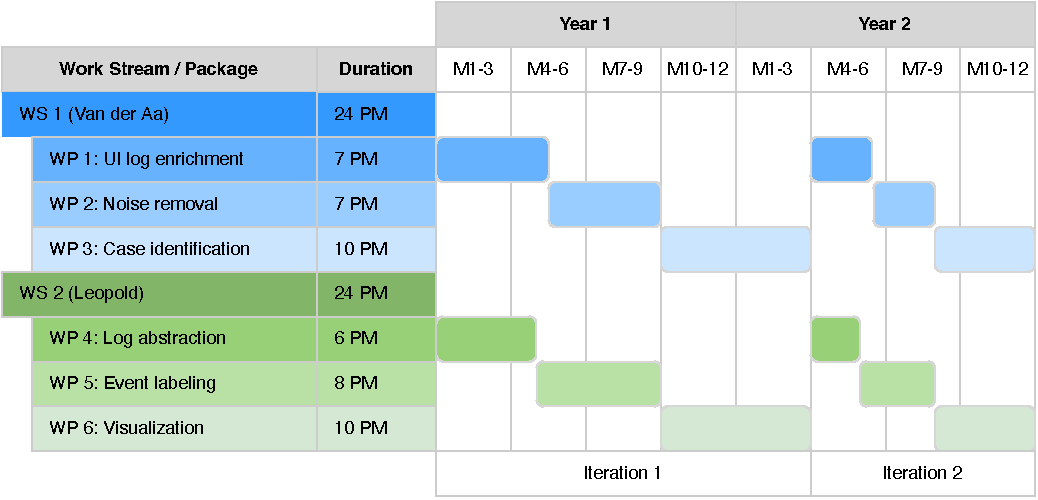
\includegraphics[width=\textwidth]{Figures/Gantt.pdf}
\caption{Work plan}
\label{fig:workplan}
\end{figure}

As explained above, the project consists of two work streams and six work packages. Naturally, there are interdependencies among these work packages. Figure \ref{fig:workplan} shows a simplified work plan that mostly abstracts from parallel and overlapping work within each work stream. It is important to highlight that the transitions between two packages will not be as strict as depicted. We are aware of the various interdependencies and will take them into account appropriately.  
There are, for instance, interdependencies between WP1 and WP1. Without an enriched UI log, the noise removal technique cannot build on the newly introduce attributes. This, however, can be addressed by taking the manually created gold standard for the evaluation of WP1 as input for WP2. In this way, the noise removal technique cannot already be developed without needing a ``perfect'' solution for WP1. The rather abstract view on the work plan shown in Figure \ref{fig:workplan} highlights our general idea of having two main iterations:
\begin{itemize}
\item The first iteration ends after 21 month. At the end of this iteration, there will be a first implemented prototype available. The individual techniques have been evaluated both independently and as a whole. The main outcome from this iteration, therefore, are insights into the strengths and weaknesses of our techniques, which allows us to determine the required improvements and adaptations for the second iteration. 
\item The second iteration is slightly shorter and will be mainly used to address identified weaknesses and improve the performance of the technique.
\end{itemize} 

Note that these two iterations also help us to account for the interdependencies between the two work streams (as discussed earlier). In the first iteration, WS 2 will build on traditional, freely available event logs, while in the second iteration WS 2 can build on a UI log that has been processed with the techniques from WS1. 



%Note that the work plan shown above allocates a total of 42 project months to 3 years. As explained in Section \ref{sec:staff}, we intend to hire a PhD student for 3 years, which means that remaining 6 project months will be covered by the respective principal investigator of this project. 

% ++++++ SECTION 3 ++++++
\section{Bibliography concerning the state of the art, the research objectives, and the work}
\printbibliography[heading=none]


% ++++++ SECTION 4 ++++++
\section{Relevance of sex, gender and/or diversity}

Neither sex, gender nor diversity will play a role in the context of this research. 
\todo{Sections 1 to 4 must not exceed 15 pages.}
\pagebreak

% ++++++ SECTION 5 ++++++
\section{Supplementary information on the research context}
% max 10 pages

 \subsection{Ethical and/or legal aspects of the project}

%We would like to stress two ethical aspects with respect to the use of social media data. First, we will only use fully legal means (e.g, by using the official Twitter API) to obtain social media data. Second, we will replace the user names associated with the extracted posts with identifiers, such that the privacy of the users is protected (even though we will only use public posts). 

\subsection{Data handling}

%As explained in Section \ref{sec:objectives} and \ref{sec:wp6}, we plan to create new data sets consisting of event logs and related Twitter posts. Such data sets are not only relevant for this project, but also for other researchers in the area of process mining. In fact, the large interest in event logs has led to the creation of a central event log repository\footnote{https://www.tf-pm.org/resources/logs}, which is hosted and managed by the IEEE Task Force on Process Mining. As a member of the IEEE Task Force on Process Mining, we therefore plan to make our data sets publicly available via this repository. 

\subsection{Other information}

All relevant information is discussed above. 

% ++++++ SECTION 6 ++++++
\section{People/collaborations/funding}


\subsection{Employment status information}

Prof. Dr. Henrik Leopold, Associate Professor at the Kühne Logistics University, permanent position.\\
Prof. Dr. Han van der Aa, Junior Professor (W1) at the University of Mannheim. Six year contract (ending in March 2026) with an interim evaluation in March 2023.

\subsection{First-time proposal data}

Not applicable.

\subsection{Composition of the project group}

\todo{We obviously need to rewrite this in a smart way. I think we should particularly focus on the complementary aspects. They should not conclude that anyone of us could do this without the other. Highlighting the successful collaboration makes sense obviously.}


The applicants of this proposal have history of successful collaboration. While they share a similar background with respect to the application of natural language processing in process analysis and mining, they both have complementary skills and knowledge. 

\textbf{Prof. Dr. Henrik Leopold} - Henrik Leopold is a tenured Associate Professor at the K\"uhne Logistics University (KLU) and senior researcher at the Hasso Plattner Institute (HPI) at the Digital Engineering Faculty, University of Potsdam. Before joining KLU/HPI in February 2019, he held positions as an Assistant Professor at the Vrije Universiteit Amsterdam (February 2015 – January 2019) and WU Vienna (April 2014 – January 2015) as well as a postdoctoral research fellow at the Humboldt University of Berlin (July 2013 – March 2014). In July 2013, he obtained a PhD degree (Dr. rer. pol.) in Information Systems from the Humboldt University of Berlin. For his thesis he received the TARGION Dissertation Award 2014 for the best doctoral thesis in the field of Information Management and the runner-up of the McKinsey Business Technology Award 2013. Henrik Leopold's research is concerned with leveraging technology from the field of artificial intelligence to develop automated techniques for process analysis and process mining. The results of his research have been published in over 80 publications in books, book chapters, journals, conferences, workshops, and reports. Among others, his research has been published in the journals IEEE Transactions on Knowledge and Data Engineering, IEEE Transactions on Software Engineering, ACM Transactions on Management Information Systems, Decision Support Systems, and Information Systems. 

\textbf{Prof. Dr. Han van der Aa} - Han van der Aa is a Junior Professor (W1) in School of Business Informatics at the University of Mannheim, where he heads the research group on process analytics since April 2020. Before that, he was an Alexander von Humboldt Fellow, working as a postdoctoral researcher in the Department of Computer Science at the Humboldt-Universität zu Berlin (May 2018 - March 2020). He obtained a PhD in computer science from the Vrije Universiteit Amsterdam in January 2018. His research interests include business process modeling, process mining, natural language processing, and complex event processing. 
The results of his research have so far resulted in close 50 publications, including articles in 
renowned international journals such as IEEE TKDE, DSS, and Information Systems, as well as at the CAISE, BPM, SIGMOD, and COLING conferences.
He is a PC member of established conferences such as BPM, ICPM, and DEBS.

\todo{Conclude by highlighting the complementary aspects.}

\subsection{Researchers in Germany with whom you have agreed to cooperate on this project}
\label{sec:collab:germany}

We agreed to cooperate on this project with three researchers from Germany: Prof. Dr. Stefanie Rinderle-Ma, Prof. Dr. Matthias Weidlich, Prof. Dr. Simone Ponzetto. 

\textbf{Prof. Dr. Stefanie Rinderle-Ma}: 

 
\textbf{Prof. Dr. Matthias Weidlich}: Matthias Weidlich is a full professor at the Department of Computer Science at Humboldt- Universi\"at zu Berlin and has been an Emmy Noether Research group leader at the same institute. Before that, he held positions at the Department of Computing at Imperial College London and at the Technion - Israel Institute of Technology. He holds a PhD from the Hasso Plattner Institute (HPI), University of Potsdam. His research focuses on process-oriented and event-driven systems and his results appear regularly in the premier conferences (VLDB, SIGMOD) and journals (TKDE, Inf. Sys., VLDBJ) in the field.

\textbf{Prof. Dr. Simone Ponzetto}: Simone Ponzetto is a professor of Information Systems at the University of Mannheim, where he leads the Natural Language Processing (NLP) and Information Retrieval group. His main research interests lie in the areas of knowledge acquisition, text understanding, and the application of NLP methods for research in the (digital) humanities and (computational) social sciences. Simone regularly serves as area chair and program committee member of *ACL and (IJC/AA)AI conferences and is an editorial board member of the Artificial Intelligence Journal and Journal of Natural Language Engineering. He is (co-)author and (co-)editor of over 100 refereed papers in scientific journals, books, and conference proceedings.

We have already collaborated with all three researchers mentioned above in the context of various research efforts. 
With Prof. Dr. Stefanie Rinderle-Ma, we worked, among others, on extracting process information from textual resources \cite{winter2020assessing}. 
With Prof. Dr. Matthias Weidlich, we worked various topics related to process mining \cite{} and low level event data \cite{}
With Prof. Dr. Simone Ponzetto, we have on ongoing cooperation on extraction of process information from text.

Based on these experiences, we are confident that both can provide valuable input for this project. With respect to the work packages, we expect \todo{finish}.


\subsection{Researchers abroad with whom you have agreed to cooperate on this project}
\label{sec:collab:abroad}

Outside Germany, we agreed to cooperate with Prof. Dr. Josep Carmona, Dr. Chiara Ghidini

 \todo{To be filled.}

\textbf{Prof. Dr. Josep Carmona}: Josep Carmona is an Associate Professor at Universitat Politècnica de Catalunya (UPC). He received a PhD at the same university in 2004, under the supervision of Prof. Jordi Cortadella. His research interests include formal methods and concurrent systems, data and process science, business intelligence and business process management, and natural language processing. He has co-authored numerous research papers and organized various conferences and workshops. He is a founder of the International Conference on Process Mining, where he is part of the Steering Committee, and a member of the IEEE Task Force on Process Mining.

%Prof.\ Carmona has conducted various works on the intersection of NLP and process analysis, including a collaboration with the applicant on the comparison of textual process descriptions to process models~\cite{sanchez2018aligning}. 


%
%\textbf{Prof. Dr. Hajo A. Reijers} - Hajo Reijers is a Full Professor in the Department of Information and Computing Sciences of Utrecht University, where he holds the chair in Business Process Management and Analytics. He is also a part-time, full professor in the Department of Mathematics and Computer Science of Eindhoven University of Technology, as well as an adjunct professor in the School of Information Systems of Queensland University of Technology (QUT). The focus of his academic research is on business process innovation, process analytics, robotic process automation, and enterprise IT. He published in Information Systems, the Journal of Management Information Systems, the Journal of Information Technology, the International Journal of Cooperative Information Systems, Organization Studies, and Omega, among other journals.
%
%Also with Prof. Dr. Hajo A. Reijers we have already worked on numerous research efforts in the area of process mining \cite{Koorn2020,van2019efficient} and NLP in process analysis \cite{van2017transforming,vanderaa2016comparing,leopold2019using}. What is more, we have worked (and are currently working) together on several research projects funded by the Dutch Research Council (NWO): 
%\begin{itemize}
%\item AutoDrivE - Automatic Derivation of Event Logs  (2019 - 2023)
%\item TACTICS - Techniques for the Analysis of Client-Team Interactions (2017 - 2022)
%\item SADIQ - Software for the Analysis of Dental Implant Quality (2016 - 2017)
%\end{itemize}
%
%Against this background, we believe that the coorporation with Prof. Dr. Hajo A. Reijers will be a valuable addition to this project. 

\subsection{Researchers with whom you have collaborated scientifically within the past three years}

\todo{To be filled.}

The researchers listed above are also the ones we have mainly collaborated with over the last three years. We plan to use this project to continue and deepen these collaborations. Other research collaborations in the context of process mining, process analysis, and natural language processing have been conducted with the following researchers:

Han:

\begin{itemize}
\item Prof Dr. Avigdor Gal (Israel Institute of Technology): Process mining
\item Prof. Dr. Jan Mendling (WU Vienna): NLP-based process analysis 
\item Prof. Dr. Heiner Stuckenschmidt 
\item Farbricio  Maggi:
\item Adela
%\item Prof. Dr. Matthias Weidlich (Humboldt University of Berlin): Conformance checking and process matching
%\item Dr. Adela del-R\'{i}o-Ortega (Universidad de Sevilla): Process performance indicators
\end{itemize}

Henrik: Hajo, Flavia, Weske, 


\subsection{Project-relevant cooperation with commercial enterprises}

We do not plan to cooperate with a commercial enterprise in the context of this project. 
%However, as discussed earlier, we plan to reuse an event log we are currently creating together with the German process mining software vendor Lana Labs\footnote{https://lanalabs.com/} in the research project \textit{AutoDrivE} (Automatic Derivation of Event Logs)\footnote{https://www.nwo.nl/onderzoek-en-resultaten/programmas/open+technologieprogramma/projecten/2018/2018-16672/} funded by the Dutch Research Council (NWO).

%As discussed earlier, we plan to cooperate with the German process mining software vendor Lana Labs\footnote{https://lanalabs.com/}. The main goal of the cooperation is to jointly create an additional data set for the evaluation of the proposed technique. We have already collected experience with Lana Labs as a project partner. In the research project \textit{AutoDrivE} (Automatic Derivation of Event Logs) funded by the Dutch Research Council (NWO), we are cooperating on the topic of automated event log extraction from transactional databases. We are, therefore, confident that also the collaboration in the context of this project will be successful.   

\subsection{Project-relevant participation in commercial enterprises}

We do not have any project-relevant participation in commercial enterprises.  

\subsection{Scientific equipment}

We won't need any further scientific equipment. 

\subsection{Other submissions}

We currently have no other proposal submissions under review.  

% ++++++ SECTION 7 ++++++
\section{Requested modules/funds}
 \subsection{Basic Module}

\subsubsection{Funding for Staff}
\label{sec:staff}

We apply for two doctoral researchers (TV-L 13) for the time of 3 years to conduct the work planned for this project (36 PM). Each position will be assigned to a PhD student who will be responsible for one work stream.

\begin{funds}[funding for staff]
\positionmul{Doctoral researcher (WS1 - Van der Aa), TV-L 13, 36 months}{5700}{36}
\positionmul{Doctoral researcher (WS2 - Leopold), TV-L 13, 36 months}{5700}{36}
\end{funds}

\subsubsection{Direct Project Costs}

\subsubsubsection{Equipment up to \euro10,000, Software and Consumables}

We will not require additional hardware or software. The required infrastructure will be provided by the K\"uhne Logistics University and the University of Mannheim.

\subsubsubsection{Travel Expenses}
\label{sec:costs:travel}
The results of the project will be published and presented at national and international conferences. We plan to visit two conferences per year. Assuming an average of \euro1500 per conference, we will need 3 x 2 \euro1500 = \euro9000 per PhD student, i.e. \euro18000 in total. We plan to conduct two joint project meetings per year: one in Hamburg and one in Mannheim. This can be covered by \euro500 per trip, which means we need \euro3000 for project meetings. We further plan to visit each of our national and international project partners once over the course of the project. The trips to the national partners can be covered by \euro500 and the international partners by \euro1000. This sums up to \euro3000 and \euro4000 respectively for the entire project. A summary and the overall total required for traveling expenses are listed below. \\

\begin{funds}[travel expenses]
\positionmul{Conference visits (3 years x 2 visits x 2 researchers)}{1500}{12}
\positionmul{Project meetings (3 years x 2 visits)}{500}{6}
\positionmul{Visit national project partner (3 partners x 1 visit x 2 researchers)}{500}{6}
\positionmul{Visit international project partners (2 partners x 1 visit x 2 researchers)}{1000}{4}
\end{funds}

\subsubsubsection{Visiting Researchers}

As explained in Sections \ref{sec:collab:germany} and \ref{sec:collab:abroad}, we plan to cooperate with several national as well as international researchers. Costs of mutual visits are listed in above in Section \ref{sec:costs:travel}.

\subsubsubsection{Expenses for Laboratory Animals}

Not applicable. 

\subsubsubsection{Other Costs}

There will not be any other costs than the positions listed above. 

\subsubsubsection{Project-related publication expenses}

We do not expect any publication expenses besides the conference fees, which we already included in the travel expenses in Section \ref{sec:costs:travel}. The total for direct projects costs is listed below. 

\subsubsection{Instrumentation}

Not applicable. 

\subsection{Module Temporary Position for Principal Investigator}

Not applicable. 

\subsection{Module Replacement Funding}

Not applicable. 

% ++++++ APPENDIX ++++++
\subsection*{Appendices}

The appendix includes the applicant's CVs (\textit{CV\_PubList\_Leopold.pdf} and \textit{CV\_PubList\_VanDerAa.pdf}) with a list of their ten most important publications.  
\end{document}


